%	- present toy examples and what they are testing
%		- these should be quite good
%	- refer to UCI datasets as well-known evaluation platforms for regression

In this section, we will empirically evaluate the proposed \acp{RFSF}.
We aim to assess the following central hypothesis:
\begin{hypothesis}
	"Do \acp{RFSF} outperform \acp{RFF} (due to their increased parameter capacity)?"
	\label{hyp:rfsfAreBetter}
\end{hypothesis}
Additionally, we try to answer:
\begin{hypothesis}
	How do different initial values of the features' amplitudes affect the performance?
	\label{hyp:initialValues}
\end{hypothesis}
In the following, we will first present some implementation details (\cref{subsec:impl}) and subsequently present the experiment setup (\cref{subsec:setup}) and results (\cref{subsec:results}).


\subsection{Implementation}  \label{subsec:impl}
	We implemented \acp{RFSF} using GPyTorch\cite{jacotNeuralTangentKernel2020} and used Adam\cite{kingmaAdamMethodStochastic2017a} for maximizing the marginal log-likelihood.
	Despite the computational advantage of not having to compute (and, most importantly, invert) the Gram matrix, we implemented \acp{RFSF} directly as a GPyTorch kernel.
	This allowed a unified view and evaluation when comparing to well-known kernels like the \ac{SE} kernel.
	Also, it allowed to just modifying the existing code for \acp{RFF}, reducing the risk of implementation errors.
	We published our implementation on \href{https://github.com/fdamken/random-fourier-series-features}{GitHub}\footnote{\url{https://github.com/fdamken/random-fourier-series-features}}.
% end


\subsection{Experiment Setup}  \label{subsec:setup}
	To assess our hypothesis, we evaluate our approach on three classes of data sets: synthetic (\cref{tab:dataSynthetic}), \ac{UCI}\cite{duaUCIMachineLearning2017} (\cref{tab:dataUci}), and robotics (real data from a cartpole with the states as inputs and control signal as target).
	The model quality is measured by the \ac{RMSE} and log-likelihood on the test data (using the test/train splits provided along\cite{galDropoutBayesianApproximation2016} for a fair comparison).
	While the \ac{RMSE} on the mean measures raw predictive performance and how closely the mean follows the true data, the log-likelihood also assess the uncertainty quantification.
	For \ac{RFSF}, we assess three different initializations of the amplitudes:
	\begin{itemize}
		\item \emph{Random:}               Sampled from a uniform distribution, i.e., $\vec{a}_{0:M}, \vec{b}_{0:M} \sim \mathcal{U}(0, 1)$.
		\item \emph{\ac{ReLU}:}            Taken from the Fourier series for a periodic \ac{ReLU}, i.e., $a_m = (\tilde{T} (-1)^m - \tilde{T}) / (m^2 \pi^2)$ and $b_m = -(\tilde{T} (-1)^m) / (m \pi)$ for $m > 0$ and $a_0 = \tilde{T}/2$ and $b_0 = 0$ (see \cref{app:perelu} for further details and the derivation).
		\item \emph{\acl{SH} (\acsu{SH}):} All set to zero except for the $0$-th which are set to one, i.e., $a_0 = b_0 = 1$, $\vec{a}_{1:M} = \vec{b}_{1:M} = \vec{0}$.
	\end{itemize}
	The idea behind each is as follows.
	The random initialization is most simplistic and a baseline for the others.
	Initializing the amplitudes as (periodic) \acp{ReLU} sets the connection to kernel learning and \acp{BNN} with the \ac{ReLU} being one of the most common activation functions.
	Starting with a single harmonic similar to \acp{RFF} connects \acp{RFSF} closer to the idea behind \acp{RFF} and serves as an assessment of our hypothesis that \acp{RFSF} should have higher capacity than \acp{RFF} (i.e., if the marginal log-likelihood would not get better by touching the other amplitudes, they shall not change).

	We compare our method to the \ac{SE} and \ac{RFF} kernel.
	For some data sets (\ac{UCI} Boston, concrete, power, and yacht), we also compare to popular approaches for \acp{BNN}:
	\begin{itemize}
		\item \emph{\ac{GBLL}:}
			A \ac{BLL} \ac{NN} with Gaussian conjugate prior on the weight. With $\vec{\phi}_{\vec{\theta}}(\vec{x})$ being the parameterized features induced by the \ac{NN} and $\mat{\Lambda}_0$ being the covariance of the prior, this is equivalent to a \ac{GP} with kernel $k_{\vec{\theta}}(\vec{x}, \vec{y}) = \vec{\phi}_{\vec{\theta}}(\vec{x})^\transposed \mat{\Lambda}_0^{-1} \vec{\phi}_{\vec{\theta}}(\vec{y})$\cite{rasmussenGaussianProcessesMachine2006}.
		\item \emph{Ensemble}\cite{lakshminarayananSimpleScalablePredictive2017}
			\todo{describe}
		\item \emph{\ac{MAP}}
			\todo{describe}
	\end{itemize}
	We include results for this models for a broader comparison, however, we did not implement them ourselves and took the results from\cite{watsonLatentDerivativeBayesian2021} (with permission).

	\begin{table}
		\centering
		\begin{tabular}{lll}
			\toprule
			\textbf{Name}         & \textbf{Function}         & \textbf{Domain}                   \\ \midrule
			Cosine                & $\cos(2 \pi x)$           & $[-0.5, 0.5]$                     \\
			Heaviside\superdagger & $\Theta(x)$               & $[-0.5, 0.5]$                     \\
			Heavi-Cosine          & $\Theta(x) \cos(2 \pi x)$ & $[-0.5, 0.5]$                     \\
			Gap-Cosine            & $\cos(2 \pi x)$           & $[-0.75, -0.25) \cup (0.5, 0.75]$ \\ \bottomrule
		\end{tabular}
		\caption{
			Synthetic Data Sets;
			All data sets are augmented with additive zero-mean Gaussian noise with $\sigma^2 = \num{e-4}$.
			\superdagger{}The heaviside function is defined as $ \Theta(x) = \max\{ 0, \mathrm{sign}(x) \} $
		}
		\label{tab:dataSynthetic}
	\end{table}

	\begin{table}
		\centering
		\begin{tabular}{lll}
			\toprule
			\textbf{Name}                 & \textbf{Short Name} & \textbf{Source}\cite{duaUCIMachineLearning2017}                  \\ \midrule
			Boston Housing                & Boston              &                                                                  \\
			Concrete Compression Strength & Concrete            & \cite{yehModelingStrengthHighperformance1998}                    \\
			Combined Cycle Power Plant    & Power               & \cite{kayaLocalGlobalLearning2012,tufekciPredictionFullLoad2014} \\
			Yacht                         & Yacht               &                                                                  \\
			Energy Efficiency             & Energy              & \cite{tsanasAccurateQuantitativeEstimation2012}                  \\
			Kinematics of 8-Link Robot    & Kin8nm              &                                                                  \\
			Naval Propulsion Plants       & Naval               & \cite{coradduMachineLearningApproaches2016}                      \\
			Protein Tertiary Structure    & Protein             &                                                                  \\
			Wine Quality (Red)            & Wine                & \cite{cortezModelingWinePreferences2009}                         \\ \bottomrule
		\end{tabular}
		\caption{\acs{UCI} Data Sets}
		\label{tab:dataUci}
	\end{table}
% end

\subsection{Results}  \label{subsec:results}
	We first compare visually the quality of \acp{RFSF} to the \ac{SE} kernel on the synthetic data.
	As this data is one-dimensional, it is straightforward to plot it.
	\Cref{fig:syntheticResultPlot} (on \cpageref{fig:syntheticResultPlot}) shows the results of the aforementioned kernels on the synthetic data.
	For every data set except the Gap-Cosine, both \acp{RFSF} and the \ac{SE} kernel approximate the true function reasonably, although \ac{SE} fails to capture discontinuities (Heaviside and Heavi-Cosine) and makes them extremely smooth.
	However, both kernels exhibit a small length-scale not appropriate for the functions.
	This is visible in the roughness of the \ac{GP} samples and is especially prevailing for the \ac{SE} on the Heaviside and Heavi-Cosine data sets (\cref{fig:syntheticResultPlotSeHeaviside,fig:syntheticResultPlotSeHeaviCosine}).
	For the Gap-Cosine data set, the \ac{SE} kernel (\cref{fig:syntheticResultPlotSeGapCosine}) clearly outperforms \acp{RFSF} (\cref{fig:syntheticResultPlotRfsfGapCosine}) within the gap by actually capturing the overall trend (with the true function lying withing the confidence interval).
	This shows that \acp{RFSF} can capture non-stationary trends (cf. \cref{fig:hypercube}) opposed to the \ac{SE} kernel.

	Quantitative results for all data sets are summarized in \cref{tab:results}.
	\Cref{tab:resultsSynthetic} contains results for the synthetic data (and cartpole) and \cref{tab:resultsUciJoe} contains \ac{UCI}-results and, for a broader comparison, some results from\cite{watsonLatentDerivativeBayesian2021}.
	The results for the remaining \ac{UCI} data sets not covered in \cref{tab:resultsUciJoe} are given in \cref{tab:resultsUciRest} in appendix \cref{app:remainingResults} for brevity (the results on the reduced data sets is sufficient for the discussion).

	\subsubsection{Synthetic Data Sets}
		On synthetic data, \acp{RFSF} perform roughly equal to the \ac{SE} kernel and \acp{RFF} on the Cosine data set in term of the log-likelihood and outperform both in terms of the \ac{RMSE} (again on the Cosine data set).
		Also, they perform better on the Heaviside data set in terms of the log-likelihood.
		However, for all other metrics (log-likelihood and \ac{RMSE} of Heavi-Cosine and Gap-Cosine as well as \ac{RMSE} on Heaviside), either the \ac{SE} kernel or \acp{RFF} outperform all variants of \acp{RFSF}.

		Focusing just on the \acp{RFSF} variants, no clear trend can be determined in terms of the log-likelihood.
		For the \ac{RMSE}, however, the \ac{ReLU} initialization is (with the exception of Cosine) outperformed by one of the other variants (Random or \ac{SH}).
	% end

	\subsubsection{\acs{UCI} Data Sets}
		In terms of the log-likelihood, \acp{RFSF} are either outperformed by or equal to the \ac{SE} kernel (once) and Ensemble (once equal, twice outperformed).
		For the remaining data sets in \cref{tab:resultsUciRest} for which\cite{watsonLatentDerivativeBayesian2021} do not report results, the results are similar.
		Within the class of \acp{RFSF} variants, the Random initialization is often superior w.r.t. to log-likelihood and \ac{RMSE}.
	% end

	\subsubsection{Cartpole Data Set}
		On the cartpole data set, the \ac{SE} kernel outperforms \acp{RFSF} and \acp{RFF} in both log-likelihood and \ac{RMSE} by far.
		For the different \acp{RFSF} variants, no clear distinction (difference of more than the measurement uncertainty) is visible.
	% end

	\begin{figure*}
		\centering
%		\begin{subfigure}{0.49\linewidth}
%			\centering
%			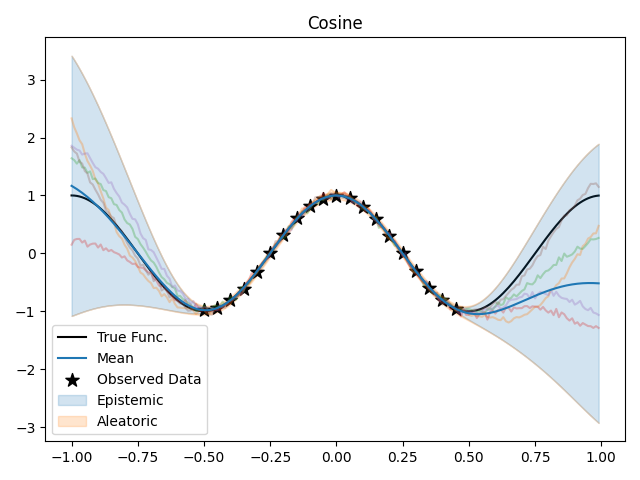
\includegraphics[width=\linewidth, height=0.618033988749895\linewidth]{graphics/generated/gp-cosine-rfsf.png}  % TODO: Replace PNG with TikZ
%			\caption{\acs{RFSF} Kernel on Cosine}
%		\end{subfigure}
%		\begin{subfigure}{0.49\linewidth}
%			\centering
%			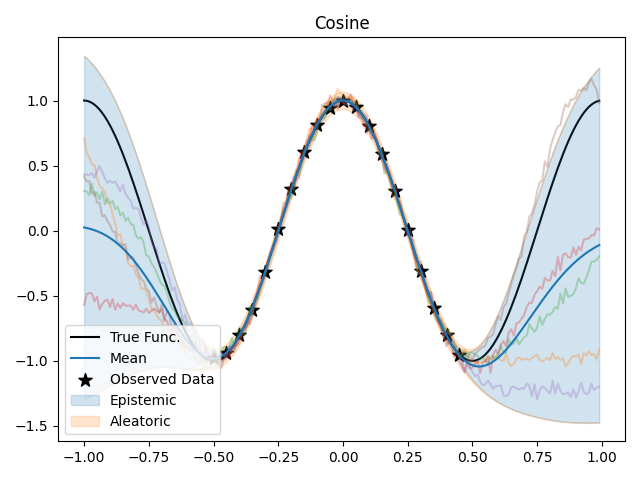
\includegraphics[width=\linewidth, height=0.618033988749895\linewidth]{graphics/generated/gp-cosine-rbf.png}  % TODO: Replace PNG with TikZ
%			\caption{\acs{SE} Kernel on Cosine}
%		\end{subfigure}
%		\\[0.5cm]
		\begin{subfigure}{0.49\linewidth}
			\centering
			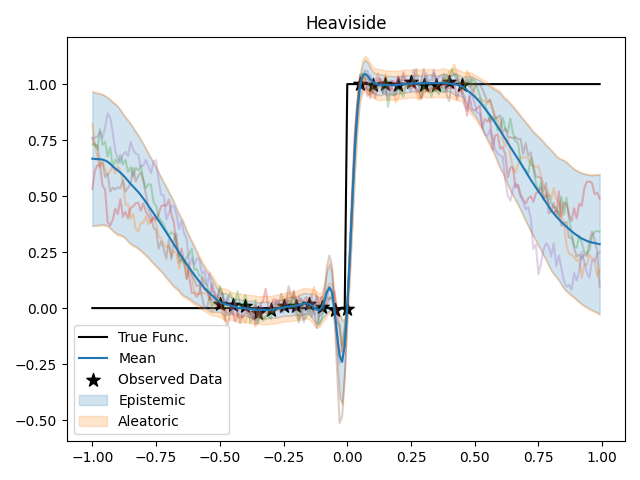
\includegraphics[width=\linewidth, height=0.618033988749895\linewidth]{graphics/generated/gp-heaviside-rfsf.png}  % TODO: Replace PNG with TikZ
			\caption{\acs{RFSF} Kernel on Heaviside}
		\end{subfigure}
		~
		\begin{subfigure}{0.49\linewidth}
			\centering
			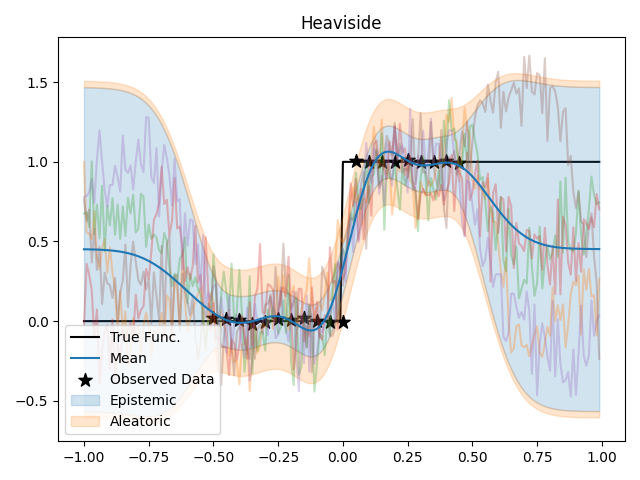
\includegraphics[width=\linewidth, height=0.618033988749895\linewidth]{graphics/generated/gp-heaviside-rbf.png}  % TODO: Replace PNG with TikZ
			\caption{\acs{SE} Kernel on Heaviside}
			\label{fig:syntheticResultPlotSeHeaviside}
		\end{subfigure}
		\\[0.5cm]
		\begin{subfigure}{0.49\linewidth}
			\centering
			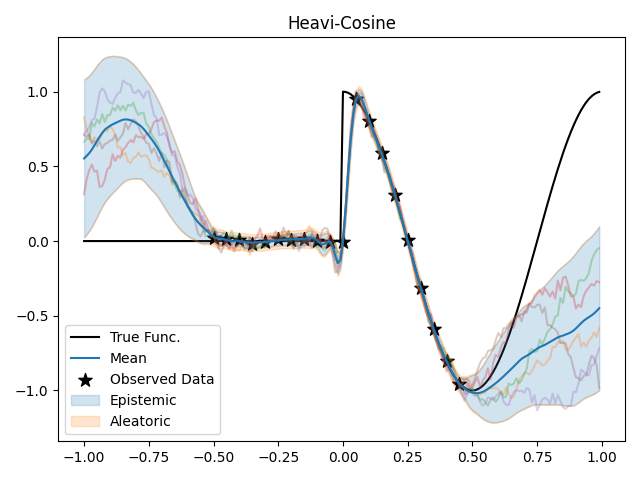
\includegraphics[width=\linewidth, height=0.618033988749895\linewidth]{graphics/generated/gp-heavicosine-rfsf.png}  % TODO: Replace PNG with TikZ
			\caption{\acs{RFSF} Kernel on Heavi-Cosine}
		\end{subfigure}
		~
		\begin{subfigure}{0.49\linewidth}
			\centering
			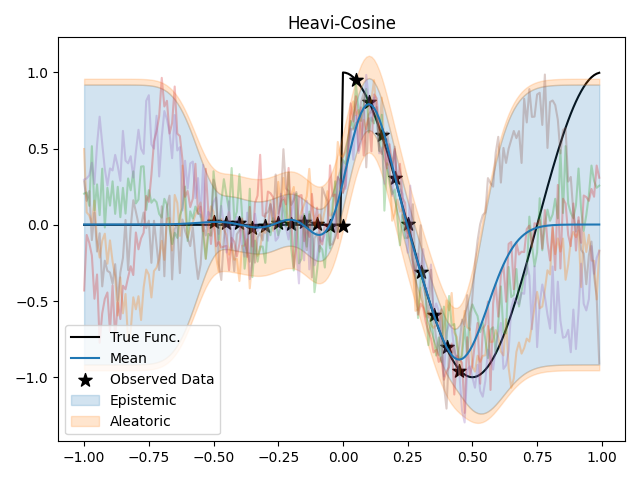
\includegraphics[width=\linewidth, height=0.618033988749895\linewidth]{graphics/generated/gp-heavicosine-rbf.png}  % TODO: Replace PNG with TikZ
			\caption{\acs{SE} Kernel on Heavi-Cosine}
			\label{fig:syntheticResultPlotSeHeaviCosine}
		\end{subfigure}
		\\[0.5cm]
		\begin{subfigure}{0.49\linewidth}
			\centering
			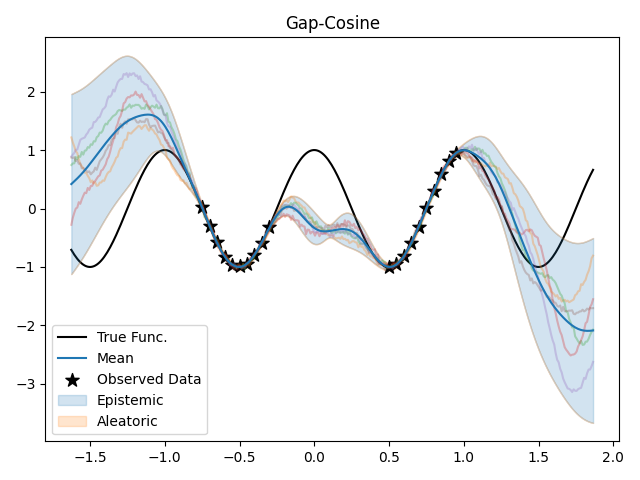
\includegraphics[width=\linewidth, height=0.618033988749895\linewidth]{graphics/generated/gp-gapcosine-rfsf.png}  % TODO: Replace PNG with TikZ
			\caption{\acs{RFSF} Kernel on Gap-Cosine}
			\label{fig:syntheticResultPlotRfsfGapCosine}
		\end{subfigure}
		~
		\begin{subfigure}{0.49\linewidth}
			\centering
			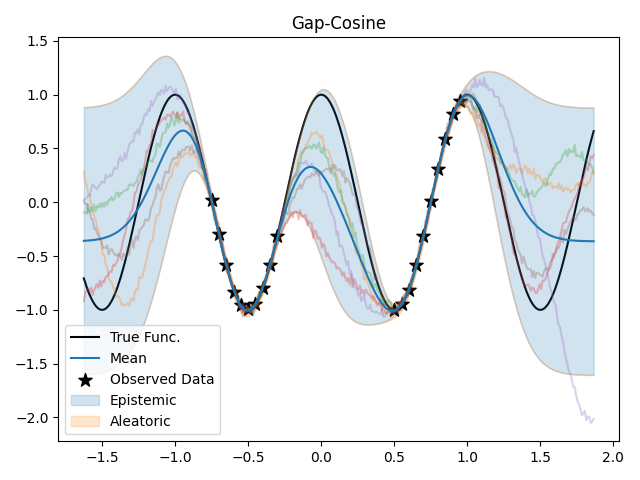
\includegraphics[width=\linewidth, height=0.618033988749895\linewidth]{graphics/generated/gp-gapcosine-rbf.png}  % TODO: Replace PNG with TikZ
			\caption{\acs{SE} Kernel on Gap-Cosine}
			\label{fig:syntheticResultPlotSeGapCosine}
		\end{subfigure}
		\caption{
			\acl{GP} regression results using an \acsp{RFSF} kernel for the synthetic data sets.
			The shaded areas depict the epistemic/aleatoric (posterior) uncertainty, the blue solid line depicts the (posterior) mean, the black stars are the training samples, and the black solid line depicts the true function.
			The colorful lines are samples from the \acsp{GP}.
			Axis labels and ticks where left out for brevity as the results are purely qualitative and specific numbers do not matter.
		}
		\label{fig:syntheticResultPlot}
	\end{figure*}

	\begin{table*}
		\centering
		\begin{subtable}{\linewidth}
			\centering
			\tabResultsSynthetic
			\caption{Results for the synthetic data sets.}
			\label{tab:resultsSynthetic}
		\end{subtable}
		\\[0.5cm]
		\begin{subtable}{\linewidth}
			\centering
			\tabResultsUciJoe
			\caption{
				Results for the \acs{UCI} datasets.
				\superdagger{}Values taken from\cite{watsonLatentDerivativeBayesian2021} with permission.
			}
			\label{tab:resultsUciJoe}
		\end{subtable}
		\caption{
			Evaluation results for the presented data sets.
			For UCI and cartpole, the mean along with the measurement uncertainty are computed over the provided train/test splits.
			The synthetic data sets only have a single train/test split, hence no uncertainty can be provided.
			Both the log-likelihood and \acs{RMSE} are reported where the higher and lower values are better, respectively.
			The best values for a data set are depicted boldface.
			Values are considered equal if their confidence regions overlap (w.r.t. the best mean value).
			The results for the remaining data sets are given in \cref{tab:resultsUciRest} in \cref{app:remainingResults}.
		}
		\label{tab:results}
	\end{table*}
% end
